\section{CMOS-Inverter}
In diesem Versuch soll der Verlauf der \"Ubertragungskennlinie und der Querstrom eines CMOS-Inverters untersucht werden.
\subsection{Experimentelle Durchf\"uhrung}
Um der CMOS-Inverter aufzubauen, wurden die Transistoren T$_{\text{n2}}$ und T$_{\text{p2}}$ des Bausteins 4007, das in der Abbildung 1 dargestellt ist, verwendet. Dabei wurde der Querstrom und die Ausgangsspannung in Abh\"angigkeit von der Eingangsspannung gemessen und schli\ss lich mit den Simulierten Ergebnisse verglichen.
\begin{figure}[!h]
\begin{center}
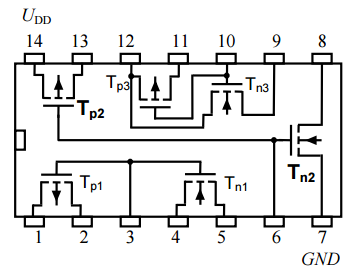
\includegraphics[scale=0.8]{bild/CMOS-Inverter}
\caption{Anschlussbelegung 4007}
\end{center}
\end{figure}
\subsection{Ergebnisse und Diskussion}
\begin{figure}[!h]
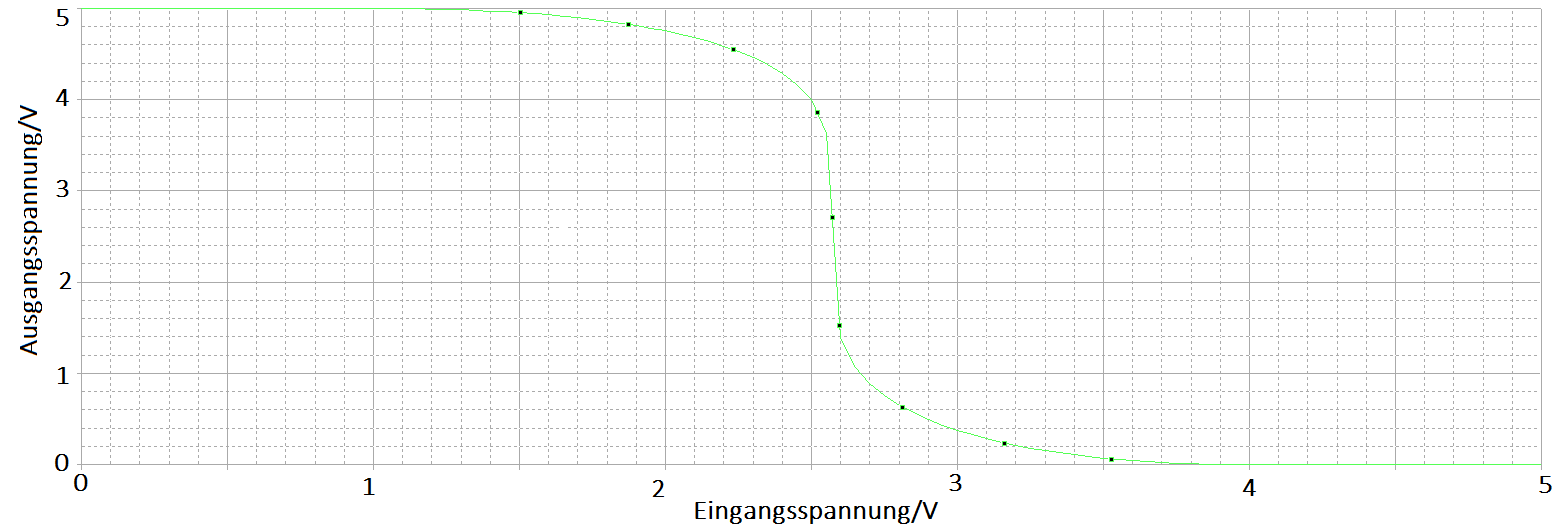
\includegraphics[scale=0.35]{bild/AusgangEingangCMOS}
\caption{Verlauf Ausgangs- zu Eingangsspannung Simulation}
\end{figure}
\begin{figure}[!h]
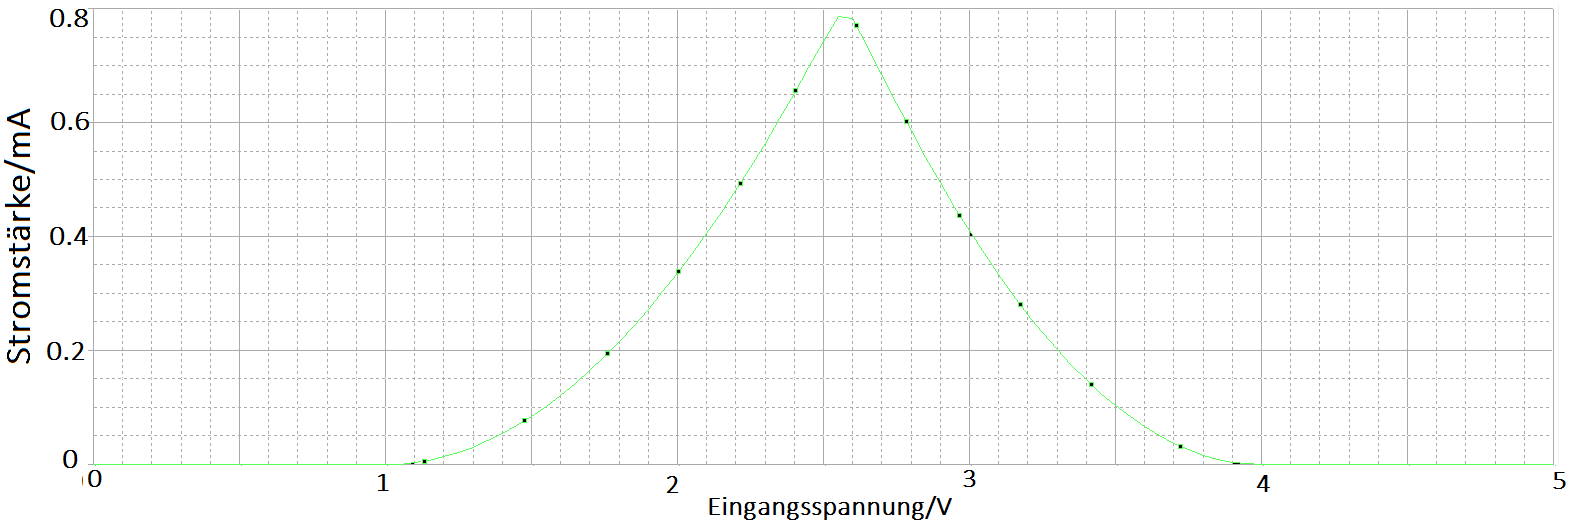
\includegraphics[scale=0.35]{bild/StromEingangCMOS}
\caption{Verlauf Strom zu Eingangsspannung Simulation}
\end{figure}